\tikzsetnextfilename{RegelvBrunFalsch}
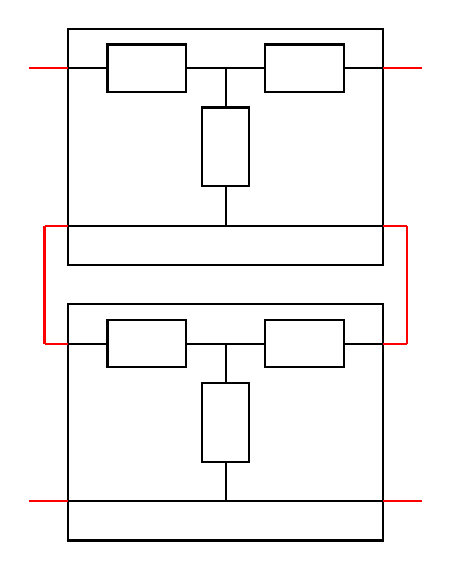
\begin{tikzpicture}[thick]
  %Unteres Viereck
  \draw (0.5,0) rectangle (4.5,3);
    \draw (0.5,0.5) -- (4.5,0.5);
    \draw (0.5,2.5) -- (1,2.5);
    \draw (2,2.5) -- (3,2.5);
    \draw (4,2.5) -- (4.5,2.5);
    \draw (1,2.8) rectangle (2,2.2);
    \draw (3,2.8) rectangle (4,2.2);
    \draw (2.5,2.5) -- (2.5,2);
    \draw (2.2,2) rectangle (2.8,1);
    \draw (2.5,0.5) -- (2.5,1);
  %Oberes Viereck
  \draw (0.5,3.5) rectangle (4.5,6.5);
      \draw (0.5,4) -- (4.5,4);
      \draw (0.5,6) -- (1,6);
      \draw (2,6) -- (3,6);
      \draw (4,6) -- (4.5,6);
      \draw (1,6.3) rectangle (2,5.7);
      \draw (3,6.3) rectangle (4,5.7);
      \draw (2.5,6) -- (2.5,5.5);
      \draw (2.2,5.5) rectangle (2.8,4.5);
      \draw (2.5,4) -- (2.5,4.5);
  %Verbindungen
    \draw [red] (0,0.5) -- (0.5,0.5);
    \draw [red] (0.2,2.5) -- (0.5,2.5);
    \draw [red] (0.2,2.5) -- (0.2,4);
    \draw [red] (0.2,4) -- (0.5,4);
    \draw [red] (0,6) -- (0.5,6);
    %Rechts
    \draw [red] (5,0.5) -- (4.5,0.5);
    \draw [red] (4.8,2.5) -- (4.5,2.5);
    \draw [red] (4.8,2.5) -- (4.8,4);
    \draw [red] (4.8,4) -- (4.5,4);
    \draw [red] (5,6) -- (4.5,6);
\end{tikzpicture}